\documentclass[xcolor={table,xdraw}]{beamer}       % presentation
% \documentclass[draft]{beamer}                    % improves compile time
% 36x24 inch poster
\usepackage[orientation=landscape,size=custom,width=100,height=60,scale=1.2,debug]{beamerposter}
\usepackage[utf8]{inputenc}                        % utf8
\usepackage[T1]{fontenc}                           % fix font encoding
\usepackage[english]{babel}                        % language
\usepackage{geometry, hyperref, fancyhdr, algorithm}
\usepackage{amsmath, amssymb, amsthm}              % ams mathematical packages
\usepackage{physics, mathtools, bm}                % extra math packages
\usepackage{xfp}                                   % floating point math
\usepackage{siunitx}                               % rounding
\usepackage[font=small]{subcaption}
\usepackage{graphicx, wrapfig}                     % images
\usepackage{booktabs, threeparttable}              % tables
\usepackage{fvextra, textcomp, CJKutf8}            % misc. text formatting
\usepackage{array}                                 % array
\usepackage[autostyle, english=american]{csquotes} % quotes
% \usepackage{tikz, pgfplots, tikz-network}          % plots and graphs
\usepackage[noend]{algpseudocode}                  % algorithm psuedocode
\usepackage[cache=true]{minted}                    % source code
\usepackage[style=ieee]{biblatex}                  % bibliography

\hypersetup{
  colorlinks=true,
  citecolor=[rgb]{0.1,0.8,0.5},
  urlcolor=cyan,
  linkcolor=magenta
}

\setminted[]{
  linenos=false,
  breaklines=true,
  encoding=utf8,
  fontsize=\normalsize,
  frame=lines,
  framesep=2mm
}

\graphicspath{{./images/}}

\def\bibfont{\scriptsize}
\addbibresource{ref.bib}

\usetheme{Szeged}
\usecolortheme{beaver}
% hide navigation buttons
\setbeamertemplate{navigation symbols}{}
% number figures
\setbeamertemplate{caption}[numbered]

% title page
\title[]{\huge Automated Musical Tempo Estimation with Neural-Network-Based Onset Detection}
\subtitle{}
\author[Stephenson]{\Large Nathan Stephenson}
\institute[TJHSST]
{
  \large TJHSST Computer Systems Lab, 2020--2021
}
\date[]{}
\titlegraphic{\vspace{-20mm}} % remove date space
\subject{Computer Science}

\begin{document}

\begin{frame}
  \maketitle
  \begin{columns}

    %%% column 1

    \begin{column}{0.33\textwidth}
      \begin{block}{Introduction} \label{sec:intro}  
        \setlength{\parindent}{1em}
        
        Tempo detection is an important technology for the synchronization of
        anything to music. Knowing the rate at which beats occur per minute
        makes it significantly more convenient to time events in music-based
        games and videos, and an automated method to find the beats per minute
        (BPM) of an audio track is especially important when precision beyond
        the human ear is necessary and when BPM needs to be calculated for more
        than a few songs, as manually determining the BPM of a track using a
        metronome and trial and error is tedious. This project explores if
        musical tempo can be determined with high accuracy through automated
        means. My method utilizes the onsets of a song, which are the starts
        of sounds or musical notes. In this paper, various tempo detection
        methods as well as various onset detection methods are assessed to
        determine which are the best fit for precision and accuracy.

      \end{block}

      \begin{block}{Background}
        \setlength{\parindent}{1em}

        \label{sec:background} A fairly unknown report was written by
        \citeauthor*{bram} \cite{bram} on tempo detection, intended for the
        purpose of synchronizing music to rhythm games. Rhythm games require the
        player to play accurately to the music, and as such the game needs to be
        able to determine if the player’s actions match with the music, making
        it important that the tempo used in the game is accurate. I found
        \citeauthor*{bram}’s method in a program he wrote called
        \href{https://arrowvortex.ddrnl.com/index.html}{ArrowVortex}
        (\url{https://arrowvortex.ddrnl.com/index.html}), which allows one to
        create rhythm game "charts," meaning synchronized instructions and
        patterns.

        Accuracy should be as close to 100\% as possible for as many songs as
        possible in order to properly synchronize anything to music, or else the
        rhythm will slowly diverge. Van de Wetering’s solution seems to show
        accurate results under the assumption that the tempo is constant in the
        music (which is true of most modern, professionally produced music) and
        that there are relatively sharp changes in the waveform (making slow
        orchestral works a bad fit, for example).  

        \begin{figure}[h!]
          \centering
          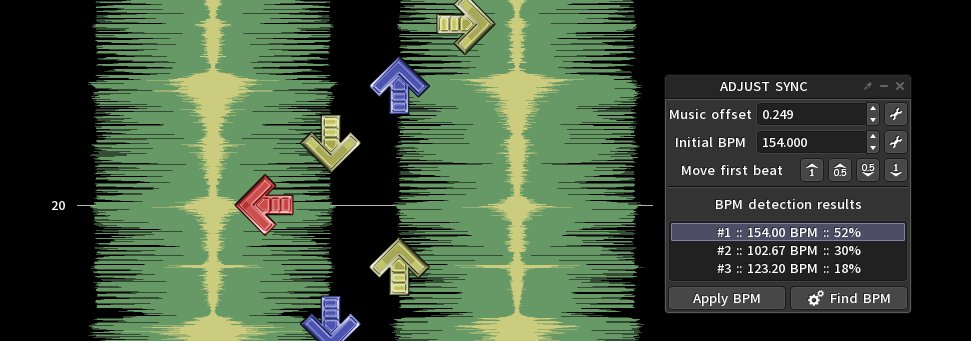
\includegraphics[scale=1]{arrowvortex}
          \caption{ArrowVortex and its sync feature.}
          \label{fig:tag}
        \end{figure}

      \end{block}

    \end{column}

    %%% column 2

    \begin{column}{0.33\textwidth}
      \begin{block}{Methods}
        \setlength{\parindent}{1em}

        A selection of 30-second samples of music were taken from Spotify for
        reference. The artists were selected mostly through Billboard's Top
        Artists of the 2010s list, though some extra artists were also added
        into the selection. The nature of the dataset suggests that the majority
        of the music being tested falls under pop or rap music, but genres such
        as country and EDM are also incorporated.

        Using \citeauthor*{bram}'s tempo detection process as a base, I compare
        various onset detection methods to see which works the best with the
        implementation. Nine algorithms will be taken from the \texttt{aubio}
        Python library, and three algorithms from the \texttt{madmom} Python
        library, all of which from the latter are neural-network-based. Spotify,
        \texttt{aubio}, and \texttt{madmom} also have their own tempo detection
        methods which I will evaluate as well.
      \end{block}

      \newcommand{\fracp}[2]{####1/####2
      (\num[round-mode=figures,round-precision=3]{\fpeval{####1/####2*100}}\%)}
      
      \begin{block}{Results}
        \begin{table}[htbp!]
            \centering
            \begin{threeparttable}
            \begin{tabular}{lllll}
            \toprule
            \textbf{Method}\tnote{1}  & \textbf{MSE}\tnote{2} & \textbf{Error rate}                     & \textbf{Insignificant errors} & \textbf{\begin{tabular}[c]{@{}l@{}}Half-BPM\\ detections\end{tabular}} \\ \midrule
            \textit{BLSTM}    & 13.813                        & \fracp{70}{773}                         & 198                           & 2                                                                      \\
            Complex           & 17.344                        & \fracp{48}{773}                         & 124                           & 1                                                                      \\
            \textit{CNN}      & \cellcolor[HTML]{EFEFEF}8.424 & \fracp{56}{773}                         & 197                           & 3                                                                      \\
            Energy            & 54.041                        & \fracp{129}{773}                        & 148                           & 10                                                                     \\
            HFC               & 44.041                        & \fracp{68}{773}                         & 120                           & 2                                                                      \\
            \textit{LL (RNN)} & 14.153                        & \cellcolor[HTML]{EFEFEF}\fracp{40}{773} & 152                           & \cellcolor[HTML]{EFEFEF}0                                              \\
            MKL               & 16.176                        & \fracp{55}{773}                         & 115                           & 2                                                                      \\
            KL                & 27.468                        & \fracp{77}{773}                         & 140                           & 2                                                                      \\
            PB                & 262.734                       & \fracp{288}{773}                        & 158                           & 33                                                                     \\
            SD                & 36.647                        & \fracp{61}{773}                         & 135                           & 6                                                                      \\
            SF                & 33.291                        & \fracp{47}{773}                         & 123                           & 1                                                                      \\
            \hline
            \texttt{aubio}    & 638.627                       & \fracp{772}{772}                        & 0                             & 130                                                                    \\
            \texttt{madmom}   & 151.536                       & \fracp{686}{772}                        & 3                             & 381                                                                    \\
            Spotify           & 116.462                       & \fracp{388}{772}                        & 376                           & 264                                                                    \\
            \bottomrule
            \end{tabular}
            \begin{tablenotes}
            \item[1] Italicized methods are neural-network-based.
            \item[2] The mode is used as ground truth.
            \item[3] Highlighted cells indicate the best value in a column. Insignificant errors are not highlighted because the best candidates in the column received the most significant errors.
            \end{tablenotes}
            \end{threeparttable}
            \caption{Comparison of various onset and tempo detection methods on the Spotify dataset.}
            \label{tab:spotifydataset}
        \end{table}
      \end{block}

    \end{column}

    %%% column 3

    \begin{column}{0.33\textwidth}

      \begin{block}{Analysis}
        \setlength{\parindent}{1em}

        Notably, none of the other tempo detection methods succeded in reaching
        comparability to \citeauthor*{bram}'s implementation. The overwhelming
        difference in error rate shows how important it is to introduce a
        working tempo detection system and open it for public use so that it is
        easier to find the correct values without doing the process by hand.
        Tempo detection for \texttt{madmom} and \texttt{aubio} was also notably
        slow; it took approximately an hour to process all the songs (1.79
        seconds per 30-second sample on average for \texttt{madmom} and
        \texttt{aubio} combined) while it took about 20 minutes to process the
        onsets and tempo for all 12 different onset methods using
        \citeauthor*{bram}'s method. In terms of performance,
        \citeauthor*{bram}'s method comparatively worked quickly.
        
        For precision, it seems that all of the neural-network-based onset
        detection algorithms are the best when detecting tempo. However, very
        slight differences in error are common and rounding is recommended to
        ensure that they work well. In terms of reliability and small error
        rates, the \textbf{Complex Domain, Spectral Flux and LL algorithms}
        shined.
        
        In terms of performance, machine-learning-based methods are naturally
        slower and more resource-intensive, though all of them work faster than
        real-time on most devices. Ultimately, Complex Domain and Spectral Flux
        seem to stand out as the best non-machine-learning based algorithms, and
        from preliminary testing it would seem that Complex Domain is more
        precise in its estimations, making that and the LL algorithm the most
        well-rounded algorithms out of the bunch, especially since both of them
        can be used in real-time as well.
       \end{block}

      \begin{block}{Conclusion}
        \setlength{\parindent}{1em}

        From looking at the previous data, it is clear that the current
        state-of-the-art tempo estimation is not perfect. Ideally the error rate
        should be as close to 0\% as possible, as projects which require
        synchronization to music need accurate tempo values. The next steps
        would be to pinpoint the weaknesses of each of the methods and create a
        large dataset with lots of variety as well as human-confirmed BPM values
        to reference. Using data from all sorts of musical genres would be
        ideal. Overall, I am pleased with the progress in this project as it is
        extremely useful to me and many others to be able to synchronize videos,
        games, and various media automatically to music without having to go
        through lengthy trial-and-error processes.
      \end{block}

      \begin{block}{References}
        \printbibliography  
      \end{block}

    \end{column}

  \end{columns}
\end{frame}
\end{document}